 \documentclass[11pt]{article}
\usepackage{parskip}
\parskip=1\baselineskip \advance\parskip by 0pt plus 2pt
\usepackage[pdftex]{graphicx}
\usepackage[utf8]{inputenc}
\usepackage[margin=1in]{geometry}
\usepackage{url}
\begin{document}

\begin{titlepage}
\begin{center}

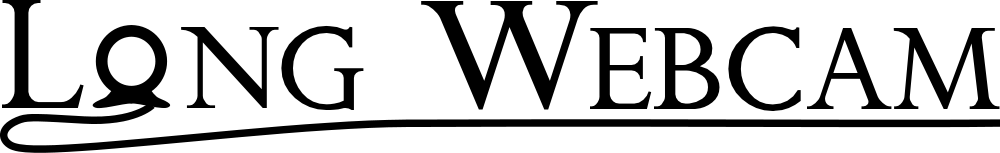
\includegraphics[width=0.85\textwidth]{./Logo_Large-cropped_black.png}

\vspace{3 cm}

\textbf{\Huge{URL-Based Camera and Weather Retrieval Program Design}}

\vspace{1 cm}

\textit{\large{Version 1.0 - 27th April 2013}}

\vspace{4 cm}

\textbf{\Large{Authors:}}

\textbf{Steve Jones} (steve@longwebcam.org)

\end{center}

\end{titlepage}

\setcounter{tocdepth}{2}
\tableofcontents
\clearpage
\pagenumbering{roman}
\section*{Document History}
    \addcontentsline{toc}{section}{Document History}
\begin{table*}[tbhp!]
\begin{tabular}{ c c p{4in} }
\textbf{Version} & \textbf{Date} & \textbf{Notes} \\
0.1 & 26 Apr 2013 & Document development; The version number will be held at 0.1 until all sections have been written. \\
1.0 & 27 Apr 2013 & Document completed
\end{tabular}
\end{table*}

\clearpage
\pagenumbering{arabic}

\section{Introduction}
This document describes the design of the program responsible for automatic retrieval of information required by the Long Webcam project from the Internet. This program will run once per hour to ensure that the required data is retrieved in a timely manner. The required information is as follows: 

\subsection{Image Retrieval}
Some of the camera images stored by the project will be taken from webcams that already publish images on the internet. The simplest way to archive such images is for the project's server to download them itself, minimising the amount of work required by the camera owner.

\subsection{Weather Retrieval}
The project will store the prevailing weather conditions alongside every image archived in the project. This information will be retrieved from World Weather Online\footnote{\protect\url{http://www.worldweatheronline.com}}.

\section{Downloading data}
\subsection{Selection of data}
The Data Retrieval program must select a number of cameras for which data must be retrieved each time it is run. The cameras will be selected using the current UTC time combined with the longitude of the camera. Using the UTC time, we can calculate the longitude where the sun is directly overhead (i.e. local midday). Any camera at a longitude within 7.5 degrees of this longitude will be selected. Weather data will be downloaded for all these cameras, regardless of how their images are retrieved. Those cameras whose images are retrieved via a URL will have their current images retrieved.

All images and weather data downloaded will be stored in the database along with a time stamp to indicate when the image was downloaded. The time stamp will be the camera's local time, together with an offset from UTC. This information will be retrieved using the Timezone API provided by World Weather Online. For remote cameras (i.e. those that are not retrieved by this Data Retrieval program), the UTC offset for the image time stamp will always be stored. When the images are uploaded from their remote locations, they will supply the local time stamp that the image was taken alongside the image itself.

\subsubsection{Retrieving previous missed data}
It is possible that in any given run of the data retrieval program that the data to be downloaded cannot be retrieved, either through network connectivity issues or faults in the web sites hosting the required data. Subsequent runs of the program will therefore locate missing data that should have been downloaded previously, and attempt to download it again. Such missing data will be marked with flags in the database, described later in this document.

The selection of the backdated data to be retrieved is slightly more complex than simply finding images and weather records that should have been downloaded but haven't. If the program attempts to download missing data indefinitely, there is a danger that it will finally succeed during the night or at the time of the next day's picture (depending on the length of the outage). Therefore, the program will only attempt to retrieve missing data on the same day as it was scheduled to be retrieved and before sunset on that day. (Calculation of the sunset time can be made based on the location of the camera and a simple geometric calculation.) If the data still cannot be downloaded after this time, it will be marked as missing, and a system alert will be raised for follow-up by one of the project staff.

\subsection{Downloading data}
Each camera selected in the query described above will be processed in turn. There will be a delay of two seconds between each camera's processing to prevent overloading of the World Weather Online API.

If the camera requires an image to be downloaded, this will be done first. The image will be retrieved from the URL, and then passed to the Image Upload Server (described in a separate document) to be added to the archive.

\subsubsection{Weather data retrieval}
Once the image has been retrieved (if required), the weather information for the camera will be obtained and added to the database.

The World Weather Online service updates its data only once every three to four hours, and each weather station covers an area of approximately 10 miles. Consequently, each time the data retrieval program wishes to download any weather data, it must look to see if that data has already been retrieved for previously. This will be achieved by searching for weather downloads using the following criteria:

\begin{itemize}
\item The camera is within 10 miles. This can be calculated using simple geometry.
\item The data was downloaded less than two hours ago
\end{itemize}

If any such data is available, it will be copied to the camera's record. Otherwise it will be downloaded from World Weather Online.

\subsubsection{Marking missing data}
For each camera image and weather record in the database, a flag will indicate whether or not the data download has been successful. (A separate flag will be used for images and weather data.) These flags will contain one of the following values:

\begin{itemize}
\item \textbf{0}: The data has been downloaded successfully
\item \textbf{1}: The data is expected to be provided soon (used for cameras whose data is uploaded from remote computers)
\item \textbf{2}: The data should have been downloaded, but could not be. Another attempt must be made
\item \textbf{3}: The data could not be downloaded, and it is now too late. The data is permanently missing
\end{itemize}

\end{document}

